\section{Output}
\label{sec:output}

When a log file is consumed by PET, the output should be usable for many
applications. On early stages of design phase or when great differences are
expected, a sparse annotated graphical output might be the best way of
visualizing power consumption. As the project evolves and more subtile changes
are evaluated, a textual output will be easier to compare. PET supports three
different output options:

\begin{description}
    \item[graph]\hfill\\
        This format is the default, and provides an overview of
        the entire program in an easily digestible format. An example of such
        a graph is printed in \autoref{fig:annot}.
    \item[plain]\hfill\\
        The example in \autoref{lst:pet_output_plain} shows the \emph{plain}
        format, which is intended to be used for further machine processing.
    \item[table]\hfill\\
        The table format, with an example shown in
        \autoref{lst:pet_output_table}, shows a terminal-printable output which
        is easier to read. It might come in handy as the default format might be
        hard to read when you are looking for specific information.
\end{description}

\subsection{Units}

The output format is understood as timeslots in which the architecture has a
certain current drain, which should be multiplied with applied voltage to get
numbers on consumed energy. The numbers are given as milliamperes, equal to
milliwatt if voltage is $1~V$. Milliamperes are used as it is easier to find
current drain rather than wattage with our setup, as described in
\autoref{sec:energymeasure}. When power is estimated for a new architecture, the
resistance of the circuit is hard to deduce, and voltage might also be an unknown
factor. Given Ohms law in \autoref{eq:ohm} and the definition of electric power
in \autoref{eq:power}

\begin{equation}
I=\frac{U}{R}
\label{eq:ohm}
\end{equation}

\begin{equation}
P=U \cdot I
\label{eq:power}
\end{equation}

it can be found that power equals current squared times resistance

\[U=R \cdot I\]
\[P=(R \cdot I) \cdot I\]
\begin{equation}
P=I^2 \cdot R
\label{eq:currentsquared}
\end{equation}
and that power equals voltage squared divided by resistance
\[P=U \cdot \frac{U}{R}\]
\begin{equation}
P=\frac{U^2}{R}
\label{eq:voltagesquared}
\end{equation}

Thus, estimating only the current drain means that the power at each point will
be unknown without knowing resistance or voltage. Further, energy comsumption
can not be estimated unless the new architecture is similar in terms of voltage
and resitance to a chip where these numbers are available. Even the current
drain might not be representable at all; if resistance or voltage is unequal
the levels found in the reference chip, the final numbers will be far off.

From \autoref{eq:currentsquared} and \autoref{eq:voltagesquared}, it is easy to
see that voltage and current is very imporant for the energy consumption. The
current is, from \autoref{eq:ohm}, dependent on resistance as well as voltage.
With this in mind, and knowing that power in a complex environment is a delicate
matter, the most important application for PET is to point in the right
direction. PET will never give accurate power estimations for new chips, but
will guide you on the way to figure out if a new feature or architectural fix
will render the final architecture more energy efficient or not.


\subsection{Examples of Output Data}

Visualization is often a good thing when inspecting old or trying to understand
new problems. \autoref{fig:annot} shows an example of PET outputting the
graphical format, with annotation.

\begin{figure}[htb]
    \centering
    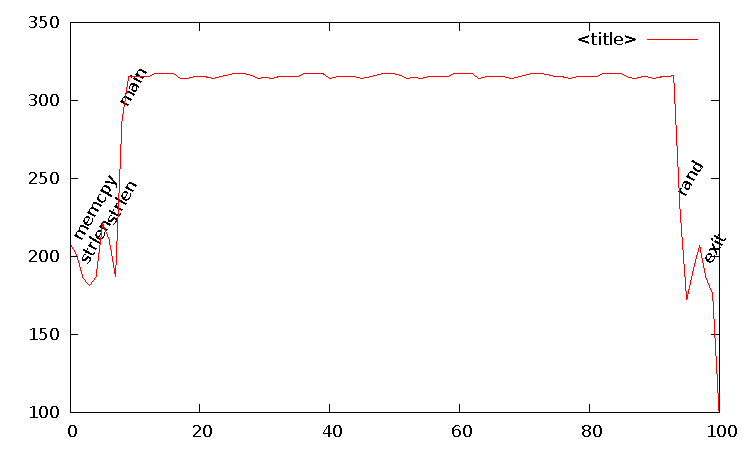
\includegraphics[width=0.9\textwidth]{figs/annot.pdf}
    \caption{PET Graphical Output. This example contains annotations, each label
    represents the entrance of a function.}
    \label{fig:annot}
\end{figure}

Example of the \texttt{plain} output format can be seen in
\autoref{lst:pet_output_plain}. The left column is the bucket number, while the
right column is instant current draw from the modelled architecture.

\begin{lstlisting}[numbers=none,float=hbt,label={lst:pet_output_plain},caption={PET plain output with function annotations.}]
0 120 memcpy
1 113 start
2 150 main
3 123 main
4 133 fun1
5 117 main
\end{lstlisting}

When reading the output directly from console, a more descriptive output format
is the \texttt{table} format. An example using this option is rendered in
\autoref{lst:pet_output_table}.

\begin{lstlisting}[numbers=none,float=hbt,label={lst:pet_output_table},caption={PET table output with function annotations.}]
/----------------------------------------\
|   Bucket   |  milliAmps |    Symbol    |
|------------|------------|--------------|
|          0 | 120.000000 |    memcpy    |
|          1 | 113.000000 |    start     |
|          2 | 150.000000 |    main      |
|          3 | 123.000000 |    main      |
|          4 | 133.000000 |    fun1      |
|          5 | 117.000000 |    main      |
\----------------------------------------/
\end{lstlisting}


